\section{Design Details}
\label{sec:impl}

In this section, we describe how we have implemented \name on Apache YARN, how we use standard techniques for demand estimation, and additional details related to our implementation.

\begin{figure}
\centering
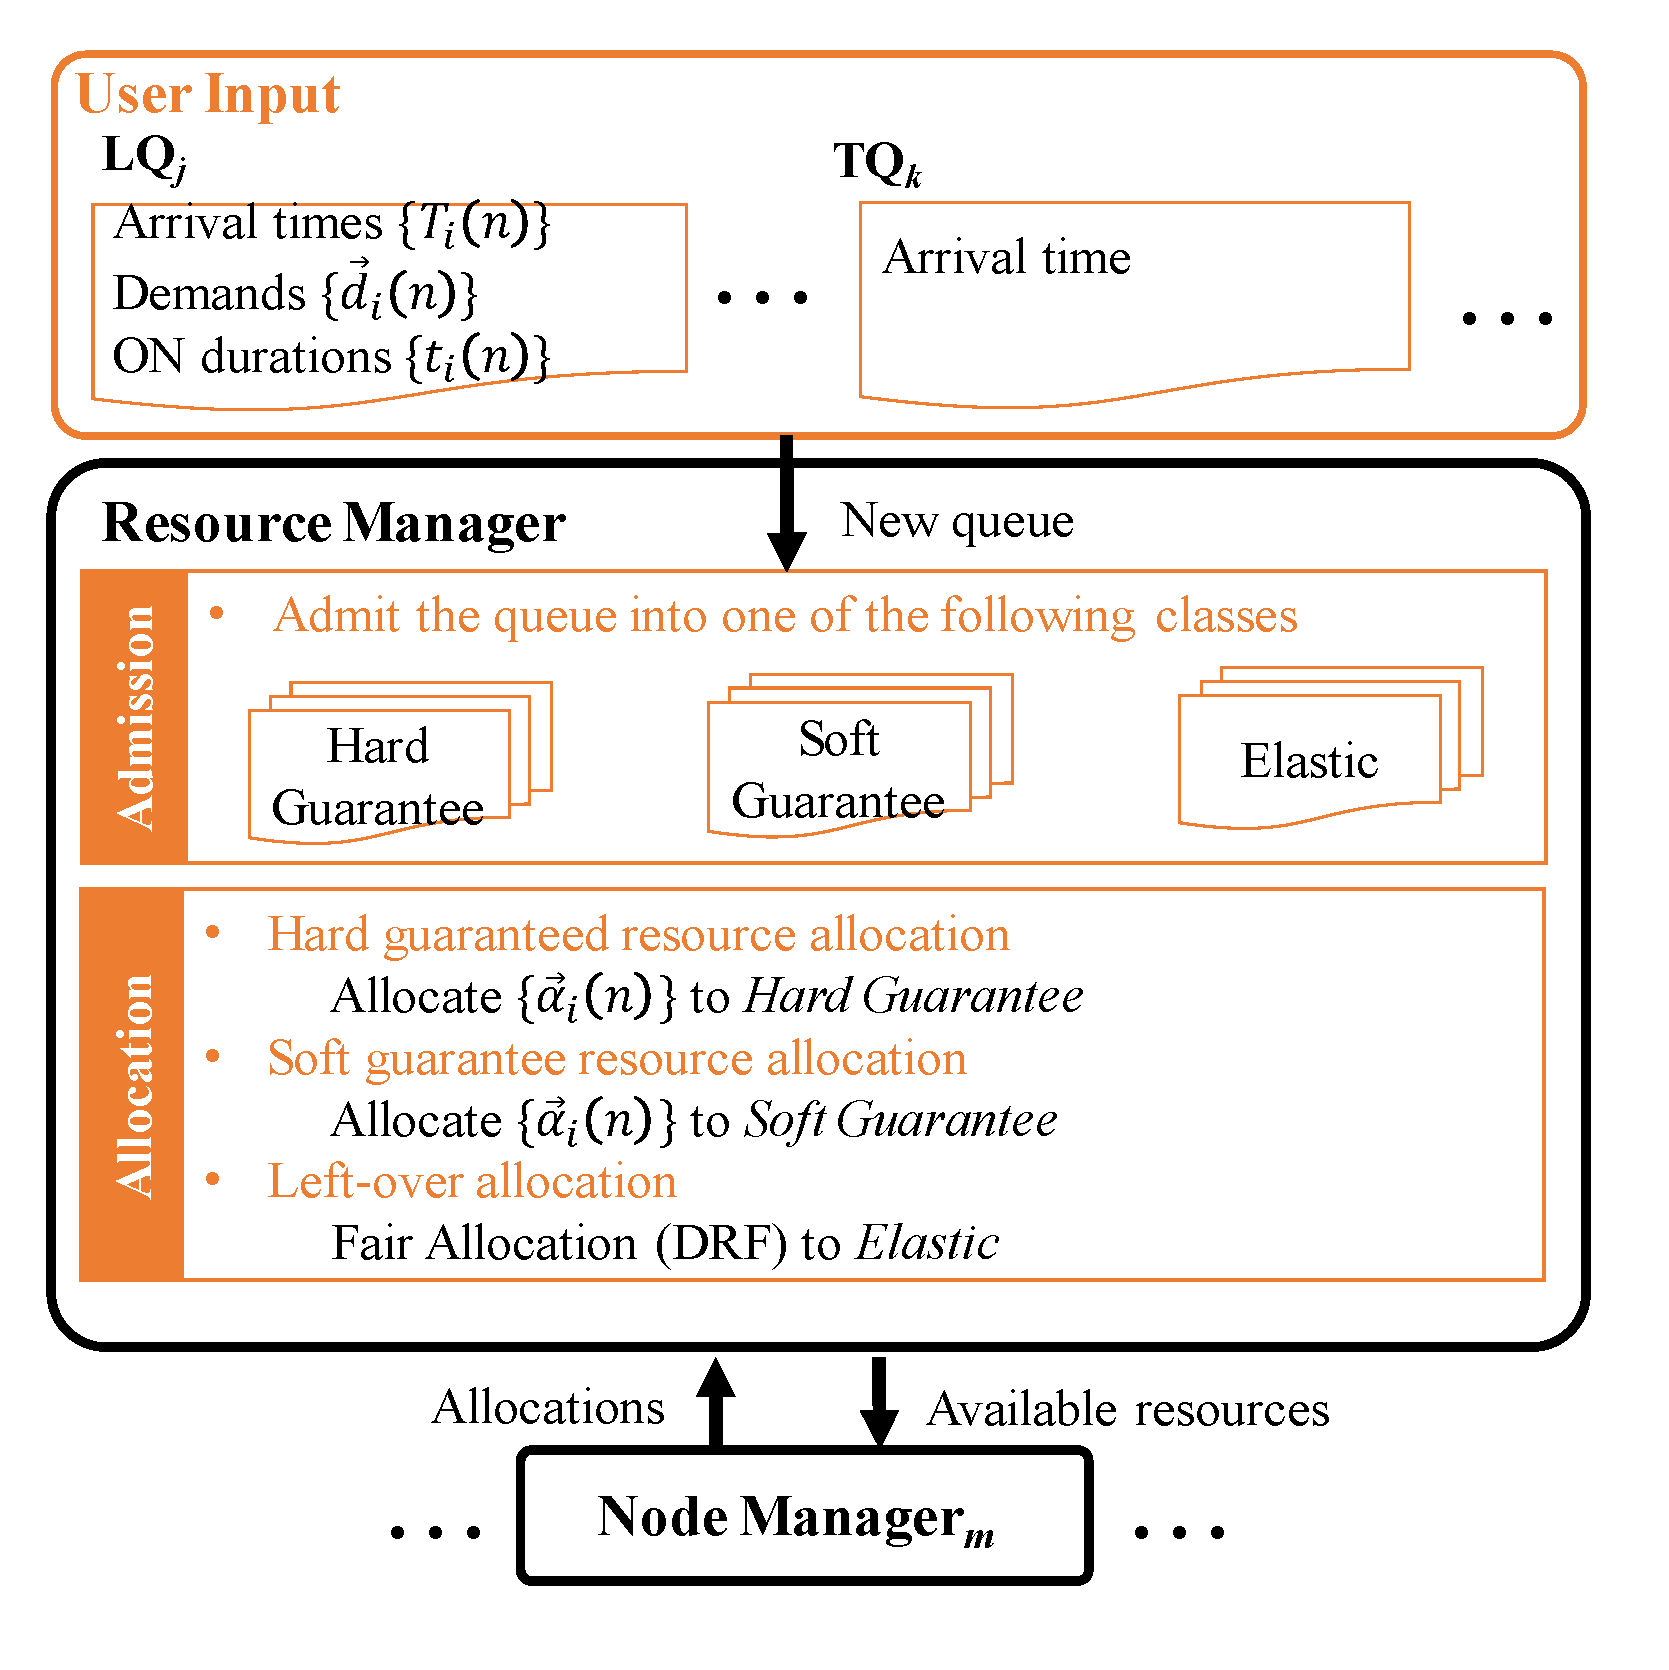
\includegraphics[width=1.0\linewidth]{fig/diagram}
\caption{Enabling bounded prioritization with long-term fairness in a  multi-resource cluster. 
\name-related changes are shown in orange. \todo{change the figure ON durations to deadlines}}
\label{fig:system_design}
\end{figure}

\subsection{Enabling \name in Cluster Managers}
Enabling bounded prioritization with long-term fairness requires implementing the \emph{\name scheduler} itself along with an additional \emph{admission control} module in cluster managers, and it takes \emph{additional information on demand characteristics} from the users. 
A key benefit of {\name} is its simplicity of implementation: we have implemented it in YARN using only $600$ lines of code.
In the following, we describe how and where we have made the necessary changes.

\subsubsection*{Primer on Data-Parallel Cluster Scheduling}
Modern cluster managers typically includes three components: \emph{job manager} or application master (AM), \emph{node manager} (NM), and \emph{resource manager} (RM).

One NM runs on each server in the cluster, and it is responsible for managing resource containers on that server. 
A container is a unit of allocation and are used to run specific tasks. 

For each application, a job manager or AM interacts with the RM to request job demands and receive allocation and progress updates. 
It can run on any server in the cluster. 
AM manages and monitors job demands (memory and CPU) and job status (\texttt{PENDING}, \texttt{IN\_PROGRESS}, or \texttt{FINISHED}). 

The RM is the most important part in terms of scheduling. 
It receives requests from AMs and then schedules resources using an operator-selected scheduling policy. 
It asks NM to prepare resource containers for the various tasks of the submitted jobs.

\subsubsection*{\name Implementation}
We made three changes for taking user input, performing admission control, and calculating resource shares -- all in the RM.
We do not modify NM and AM.
Our implementation also requires more input parameters from the users regarding the demand characteristics of their job queues. 
Figure~\ref{fig:system_design} depicts our design.

\paragraph{User Input} Users submit their jobs to their queues. 
In our system, there are 2 queue types, i.e., {\burstq}s and {\batchq}s. 
We do not need additional parameters for {\batchq}s because they are the same as the conventional queues. 
Hence, we assume that {\batchq}s are already available in the system. 
However, the \name scheduler needs additional parameters for LQs; namely, arrival times and demands.

Users submit a request job that contains their parameters of the new \burstq. 
After receiving the parameters in the job, the RM sets up a new \burstq queue for the user.
Users can also ask the cluster administrator to set up the parameters. 

\paragraph{Admission Control} YARN does not support admission control. 
We implement an admission control module to classify {\burstq}s and {\batchq}s into Hard Guarantee, Soft Guarantee, and Elastic classes. 
A new queue is rejected if it cannot meet the safety condition \eqref{eqn:ad-safety}, which invalids the committed performance.
If it is a \batchq, it is added into the Elastic class.
If the new {\burstq} does not satisfy the fairness condition \eqref{eqn:ad-fair}, it is also admitted to the Elastic class.
If the new {\burstq} meets the fairness condition \eqref{eqn:ad-fair}, but fails at the resource condition \eqref{eqn:ad-enough}, it will be put in the Soft Guarantee class.
If the new {\burstq} meets all the three conditions, i.e., safety, fairness, and resource, it will be admitted to the Hard Guarantee class.

\paragraph{\name Scheduler} We implement \name as a new scheduling policy to achieve our joint goals of bounded priority with long-term fairness. 
Upon registering the queues, users submit their jobs to their {\burstq}s or {\batchq}s. 
Thanks to admission control, {\burstq}s and {\batchq}s are classified into Hard Guarantee, Soft Guarantee, and Elastic classes. 
Note that resource sharing policies are implemented across queues in YARN, jobs in the same queue are scheduled in FIFO manner.
Hence, \name only sets the share at the individual queue level.

\name Scheduler periodically set the share levels to all {\burstq}s in Hard Guarantee and Soft Guarantee classes.
These share levels are actually upper-bounds on resource allocation that an {\burstq} can receive from the cluster. 
Based on the real demand of each {\burstq}, \name allocates resources until it meets the share levels\delete{ (whether it is in the ON period or OFF period)}. 

\name Scheduler allocates the resource to the three classes in the following priority order: (1) Hard Guarantee class, (2) Soft Guarantee class, and (3) Elastic class. 
The {\burstq}s in the Hard Guarantee class are allocated first.
Then, the \name continues allocates the resource to the {\burstq}s in Soft Guarantee class.
The queues in the Elastic class are allocated with left-over resources using DRF \cite{drf}.

%To ensure work conservation, unused resources by all queues are combined and redistributed across queues in the Elastic class using DRF \cite{drf}. 

\subsection{Demand Estimation}

\name requires accurate estimates of resource demands and their durations of \burstq jobs by users. 
These estimations can be done by using well-known techniques; \eg, users can use history of prior runs \cite{rope, jockey, tetris} with the assumption that resource requirements for the tasks in the same stage are similar \cite{drf, pacman, paratimer}. 
We do not make any new contributions on demand estimation in this paper. 
%While {\name} performs the best with accurate estimations, we have found that {\name} is robust to small misestimations in practice (\S\ref{sec:performance_large_scale}).
When LQs have bursty arrivals of different sizes, BPF with the $\alpha$-strategy ensures the performance with the average usage remains similar (\S\ref{sec:performance_large_scale}). 
We consider a more thorough study an important future work. 

\subsection{Operational Issues}

\paragraph{Container Reuse}
Container reuse is a well-known technique that is used in some application frameworks, such as Apache Tez. 
The objective of container reuse is to reduce the overheads of allocating and releasing containers. 
The downside is that it causes resource waste if the container to be reused is larger than the real demand of the new task. 
Furthermore, container reuse is not possible if the new task requires more resource than existing containers. 
For our implementation and deployment, we do not enable container reuse because {\name} periodically prefers more free resources for \burstq jobs, causing its drawbacks to outweigh its benefits in many cases.

\paragraph{Preemption}
Preemption is a recently introduced setting in the YARN Fair Scheduler \cite{hadoop-fair-scheduler}, and it is used to kill running containers of one job to create free containers for another. 
By default, preemption is not enabled in YARN. 
For {\name}, using preemption can help in providing guarantees for {\burstq}s. 
However, killing the tasks of running jobs often results in failures and significant delays. 
We do not use preemption in our system throughout this paper.

%\subsection{Possible issues}

%In the same worker node, containers are sequentially launched. Slow allocation of containers may hurt resource guarantee.

% % old text % %
%\begin{algorithm}
%\caption{Scheduler}
%\label{algorithm1}
%\begin{algorithmic}[1]
%\Procedure{periodicSchedule()}{}
%\State $\{\mathbb{A}, \mathbb{B}, \mathbb{U}\}$ = \textsc{updateQueueStatus}($\mathbb{A}$,$\mathbb{B}$,$\mathbb{U}$)
%\If{\textsc{isNewArrival}($\mathbb{Q}$)}
%	\State Update the best effort queues: $\mathbb{U} = \mathbb{U} \cup \mathbb{Q}$
%\EndIf
%\State $\{\mathbb{A}, \mathbb{B}, \mathbb{U}\}$ = \textsc{admit}($\mathbb{U}$)
%\State \textsc{allocate}($\mathbb{A}$,$\mathbb{B}$)
%\State Obtain the available cluster resources $\myvec{L}$
%\State DRF($\mathbb{U}$, $\myvec{L}$)
%\EndProcedure
%\\
%\Function{updateQueueStatus($\mathbb{A}$,$\mathbb{B}$,$\mathbb{U}$)}{}
%\ForAll{queue $A \in \mathbb{A}$}
%	\If{queue $A$ is deactivated}  Update $\mathbb{A} = \mathbb{A} \setminus A$
%	\EndIf
%\EndFor
%\ForAll{queue $B \in \mathbb{B}$}
%	\If{queue $B$ is deactivated} Update $\mathbb{B} = \mathbb{B} \setminus B$
%	\EndIf	
%\EndFor
%\ForAll{queue $U \in \mathbb{U}$}
%	\If{queue $U$ is deactivated} Update $\mathbb{U} = \mathbb{U} \setminus U$
%	\EndIf
%\EndFor
%\State \textbf{return} $\{\mathbb{A} , \mathbb{B},\mathbb{U}  \}$	
%\EndFunction
%\\
%\Function{admit(queues $\mathbb{U}$)}{}
%\ForAll{queue $U \in \mathbb{U}$}
%	\If{queue $U$ is a bursty queue}
%		\If{admission conditions \eqref{eqn:bursty_adm_cond_2} satisfied}
%			\State Update $\mathbb{A} = \mathbb{A} \cup U$
%			\State Update $\mathbb{U} = \mathbb{U} \setminus U$
%		\EndIf
%	\Else
%		\If{admission condition \eqref{eqn:batch_adm_cond} satisfied}
%			\State Update $\mathbb{B} = \mathbb{B} \cup U$
%			\State Update $\mathbb{U} = \mathbb{U} \setminus U$
%		\EndIf
%	\EndIf
%\EndFor
%\State \textbf{return} $\{\mathbb{A} , \mathbb{B},\mathbb{U}  \}$	
%\EndFunction
%\\
%\Function{\diff{allocate}($\mathbb{A}$, $\mathbb{B}$)}{}
%\ForAll{bursty queue $A \in \mathbb{A}$}
%		\State Compute $\myvec{a_i}$ allocated to queue $A$ as \eqref{eqn:alpha_1}, \eqref{eqn:alpha_2a}
%\EndFor
%\State Obtain the available cluster resources $\myvec{L}$
%\State $\myvec{R_b}$ = \textsc{DRF}($\mathbb{B}$,$\myvec{L}$) as Algorithm 1 of \cite{drf}.  
%\EndFunction
%\end{algorithmic}
%\end{algorithm}
